\chapter{Support Vector Machine}

Support Vector Machine \cite{svm} (SVM) was first heard in 1992, introduced by Boser, Guyon, and Vapnik in COLT-92. Support vector machines (SVMs) are a set of related supervised learning methods used for classification and regression. 

A Support Vector Machine (SVM) is a discriminative classifier formally defined by a separating hyperplane. In other words, given labeled training data (supervised learning), the algorithm outputs an optimal hyperplane which categorizes new examples.

Hyperplanes are decision boundaries that help classify the data points. Data points falling on either side of the hyperplane can be attributed to different classes. Also, the dimension of the hyperplane depends upon the number of features. If the number of input features is 2, then the hyperplane is just a line. If the number of input features is 3, then the hyperplane becomes a two-dimensional plane.

\section{SVM}
Suppose a training dataset is given of \(n\) points of the form \(({\vec {x}}_{1},y_{1}),\ldots ,({\vec {x}}_{n},y_{n})\) where the \(\displaystyle y_{i}\) are either 1 or -1, each indicating the class to which the point \(\displaystyle {\vec {x}}_{i}\) belongs. Each \(\displaystyle {\vec {x}}_{i}\) is a \(\displaystyle p\)-dimensional real vector. It is required to find the "maximum-margin hyperplane" that divides the group of points \(\displaystyle {\vec {x}}_{i}\) for which \(\displaystyle y_{i}=1\) from the group of points for which \(\displaystyle y_{i}=-1\), which is defined so that the distance between the hyperplane and the nearest point \(\displaystyle {\vec {x}}_{i}\) from either group is maximized.

\begin{figure}[h]
\centering
    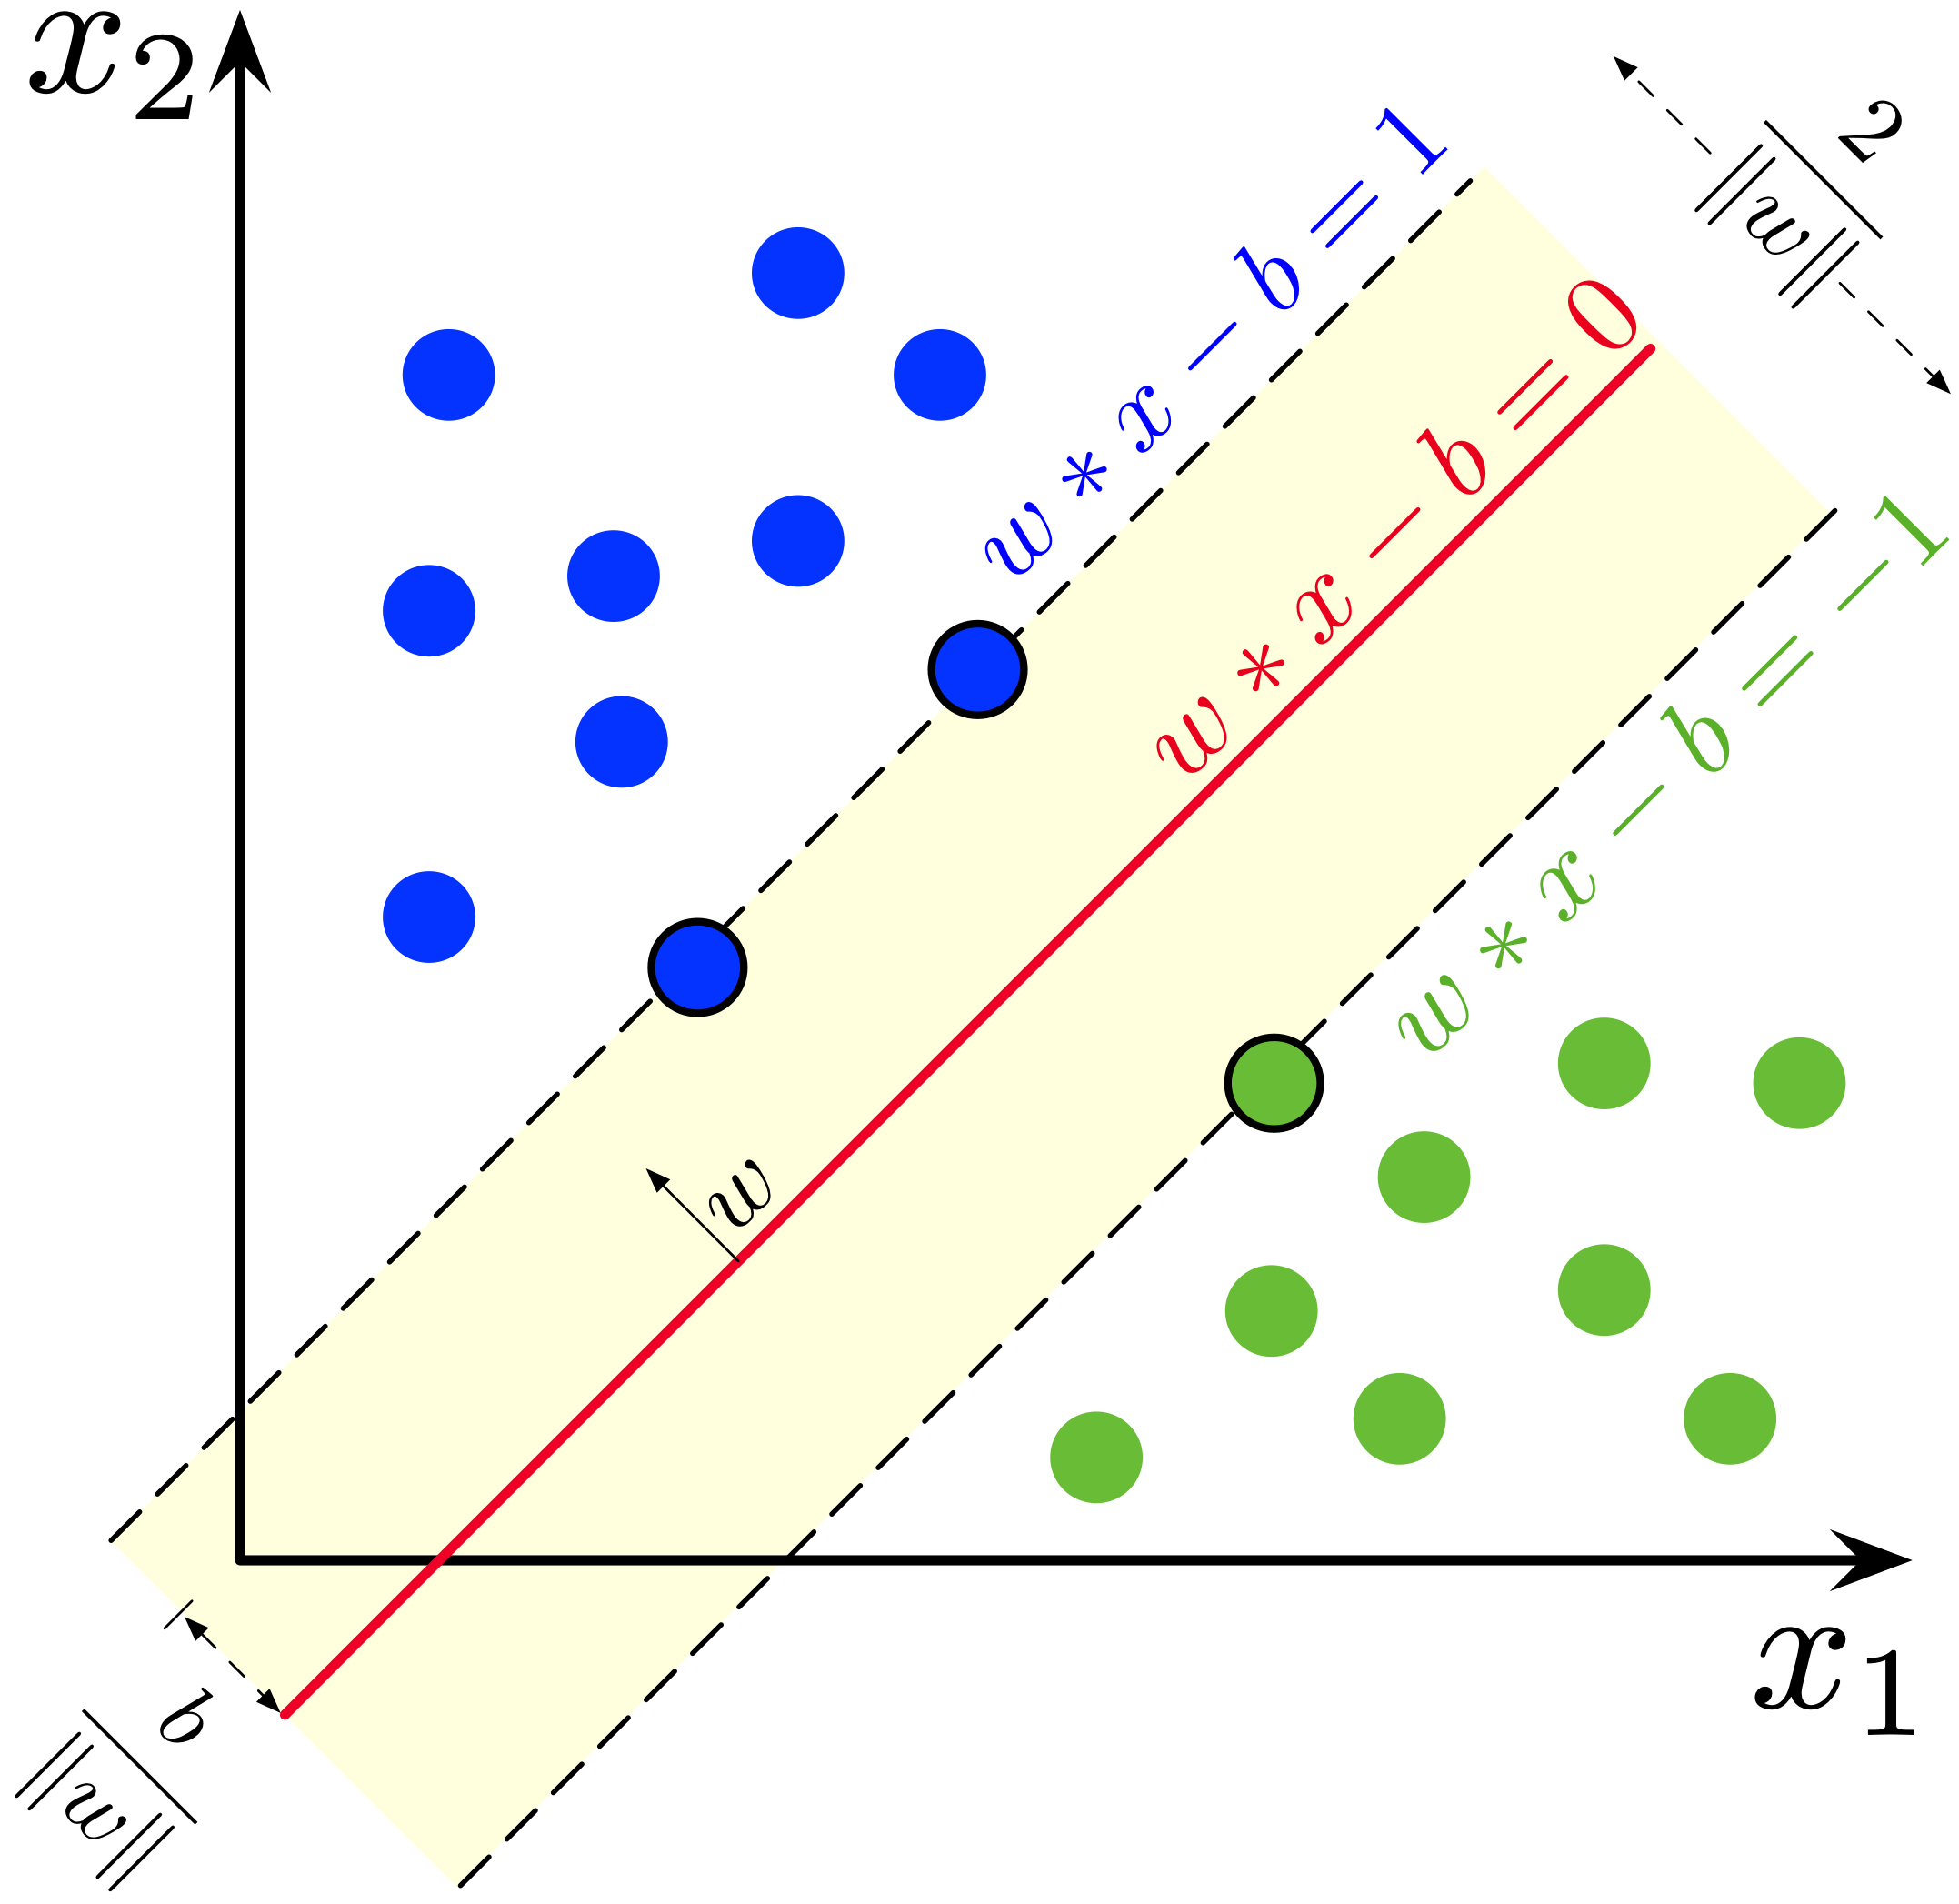
\includegraphics[scale=.5]{SVM_margin.png}
    \caption{SVM \cite{svm}}
\end{figure}

Any hyperplane can be written as the set of points \(\displaystyle {\vec {x}}_{i}\) satisfying
\begin{equation}
    {\vec {w}}\cdot {\vec {x}}-b=0
\end{equation}

where \(\displaystyle {\vec {w}}\) is the  normal vector to the hyperplane. The parameter \(\displaystyle {\frac {b} {\|{\vec {w}}\|}}\) determines the offset of the hyperplane from the origin along the normal vector \(\displaystyle {\vec {w}}\).

If the training data is linearly separable, two parallel hyperplanes can be seleted that separate the two classes of data, so that the distance between them is as large as possible. The region bounded by these two hyperplanes is called the "margin", and the maximum-margin hyperplane is the hyperplane that lies halfway between them. With a normalized or standardized dataset, these hyperplanes can be described by the equations

\begin{equation}
    {\vec {w}}\cdot {\vec {x}}-b=1    
\end{equation}

\begin{equation}
    {\vec {w}}\cdot {\vec {x}}-b=-1
\end{equation}

Equation 6.2 is for input vector \({\vec {x}}\) which is on or above this boundary to one class with label 1 and equation 6.3 is for input vector \({\vec {x}}\) which  on or below this boundary is of the other class, with label −1)

Geometrically, the distance between these two hyperplanes is \(\displaystyle {\frac {2}{\|{\vec {w}}\|}}\). To maximize the distance between the planes, \(\displaystyle \|{\vec {w}}\|\) need to be minimized. The distance is computed using the distance from a point to a plane equation. It is also required to prevent data points from falling into the margin, hence the following constraint is added : 

\begin{equation}
    {\vec {w}}\cdot {\vec {x}}_{i}-b\geq 1\) \quad if \quad\( y_{i}=1
\end{equation}
    
\begin{equation}
    {\vec {w}}\cdot {\vec {x}}_{i}-b\leq -1\) \quad if\quad \(y_{i}=-1
\end{equation}

These constraints state that each data point must lie on the correct side of the margin. Equations 6.4 and 6.5 can be combined  and  rewritten as

\begin{equation}
    y_{i}({\vec {w}}\cdot {\vec {x}}_{i}-b)\geq 1,\quad \forall \quad 1\leq i\leq n.\qquad \qquad    
\end{equation}

This can be combined together to get the optimization problem:
"Minimize \(\|{\vec {w}}\|\) subject to \(y_{i}({\vec {w}}\cdot {\vec {x}}_{i}-b)\geq 1\) for \( i=1,\ldots ,n\)".
The \({\vec {w}}\) and b that solve this problem determine the required classifier, \({\vec {x}}\mapsto \operatorname {sgn}({\vec {w}}\cdot {\vec {x}}-b)\).

An important consequence of this geometric description is that the max-margin hyperplane is completely determined by those \({\vec {x}}_{i}\) that lie nearest to it. These \( {\vec {x}}_{i}\) are called support vectors.
\newpage